%
% --- inline annotations
%
\newcommand{\red}[1]{{\color{red}#1}}
\newcommand{\todo}[1]{{\color{red}#1}}
\newcommand{\TODO}[1]{\textbf{\color{red}[TODO: #1]}}
\newcommand{\TF}[1]{\textcolor{purple}{#1}}
\newcommand{\LK}[1]{\textcolor{blue}{#1}}
\newcommand{\T}[1]{\textcolor{red}{#1}}
\newcommand{\YKL}[1]{\textcolor{red}{#1}}
\newcommand{\name}[0]{OmniTrack}
% --- disable by uncommenting  
% \renewcommand{\TODO}[1]{}
% \renewcommand{\todo}[1]{#1}

\makeatletter
\newcommand{\algorithmfootnote}[2][\footnotesize]{%
  \let\old@algocf@finish\@algocf@finish% Store algorithm finish macro
  \def\@algocf@finish{\old@algocf@finish% Update finish macro to insert "footnote"
    \leavevmode\rlap{\begin{minipage}{\linewidth}
    #1#2
    \end{minipage}}%
  }%
}
\makeatother


\makeatletter
\newcommand{\shortcline}[1]{%
  \noalign{\global\advance\@totalleftmargin by 0.15em}% 调整左缩进
  \noalign{\global\advance\linewidth by -10em}% 调整右缩进
  \cline{#1}%
  \noalign{\global\advance\@totalleftmargin by -0.5em}% 恢复左缩进
  \noalign{\global\advance\linewidth by 1em}% 恢复右缩进
}
\makeatother


\definecolor{codegreen}{rgb}{0.0,0.6,0.0}
\definecolor{mygray}{gray}{.9}
\definecolor{mygray1}{gray}{.7}
\definecolor{tabgray}{rgb}{0.957,0.945,0.925}


% icon
\newcommand{\car}{
\includegraphics[width=4mm]{imgs/icon/car2.png}}
\newcommand{\robot}{
\includegraphics[width=4mm]{imgs/icon/robot.png}}
\newcommand{\robotdog}{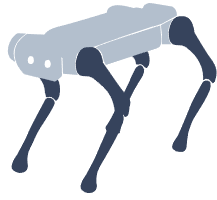
\includegraphics[width=4mm]{imgs/icon/robotDog.png}}
\newcommand{\webm}{
\includegraphics[width=3.6mm]{imgs/icon/webm.png}}
\newcommand{\mywebm}{
\includegraphics[width=3.5mm]{imgs/icon/webm2.png}}

\newcommand{\wheels}{
\includegraphics[width=4mm]{imgs/icon/wheels.png}}
\newcommand{\gait}{
\includegraphics[width=4mm]{imgs/icon/gait.png}}
\newcommand{\stationary}{
\includegraphics[width=4mm]{imgs/icon/stationary2.png}}

\newcommand{\mycheckmark}{
\includegraphics[width=3.5mm]{imgs/icon/checkmark.png}}
\newcommand{\crossmark}{
\includegraphics[width=3.5mm]{imgs/icon/crossmark.png}}


\newcommand{\topline}{\noalign{\hrule height 0.8 pt}} 
\newcommand{\midline}{\noalign{\hrule height 0.6 pt}} 
\newcommand{\bottomline}{\noalign{\hrule height 0.8 pt}} 

\definecolor{codebackgroundcolor}{RGB}{248,242,222}

%

\definecolor{r1}{rgb}{0.7569,0.2275,0.1294}
\definecolor{r2}{rgb}{0.0,0.5451,0.5451}
\definecolor{r3}{rgb}{0.5451,0.0,0.5451}

\newcommand{\ROne}{\textit{\textcolor{r1}{R1}}}
\newcommand{\RTwo}{\textit{\textcolor{r2}{R2}}}
\newcommand{\RThree}{\textit{\textcolor{r3}{R3}}}


\def\maketitlesupplementaryfinal
   {
   \newpage
       \twocolumn[
        \centering
        \Large
        \textbf{Supplementary Materials for \thetitle}\\
        \vspace{1.0em}
       ] %< twocolumn
   }

